% Created by tikzDevice version 0.6.1 on 2011-08-02 12:46:19
% !TEX encoding = UTF-8 Unicode
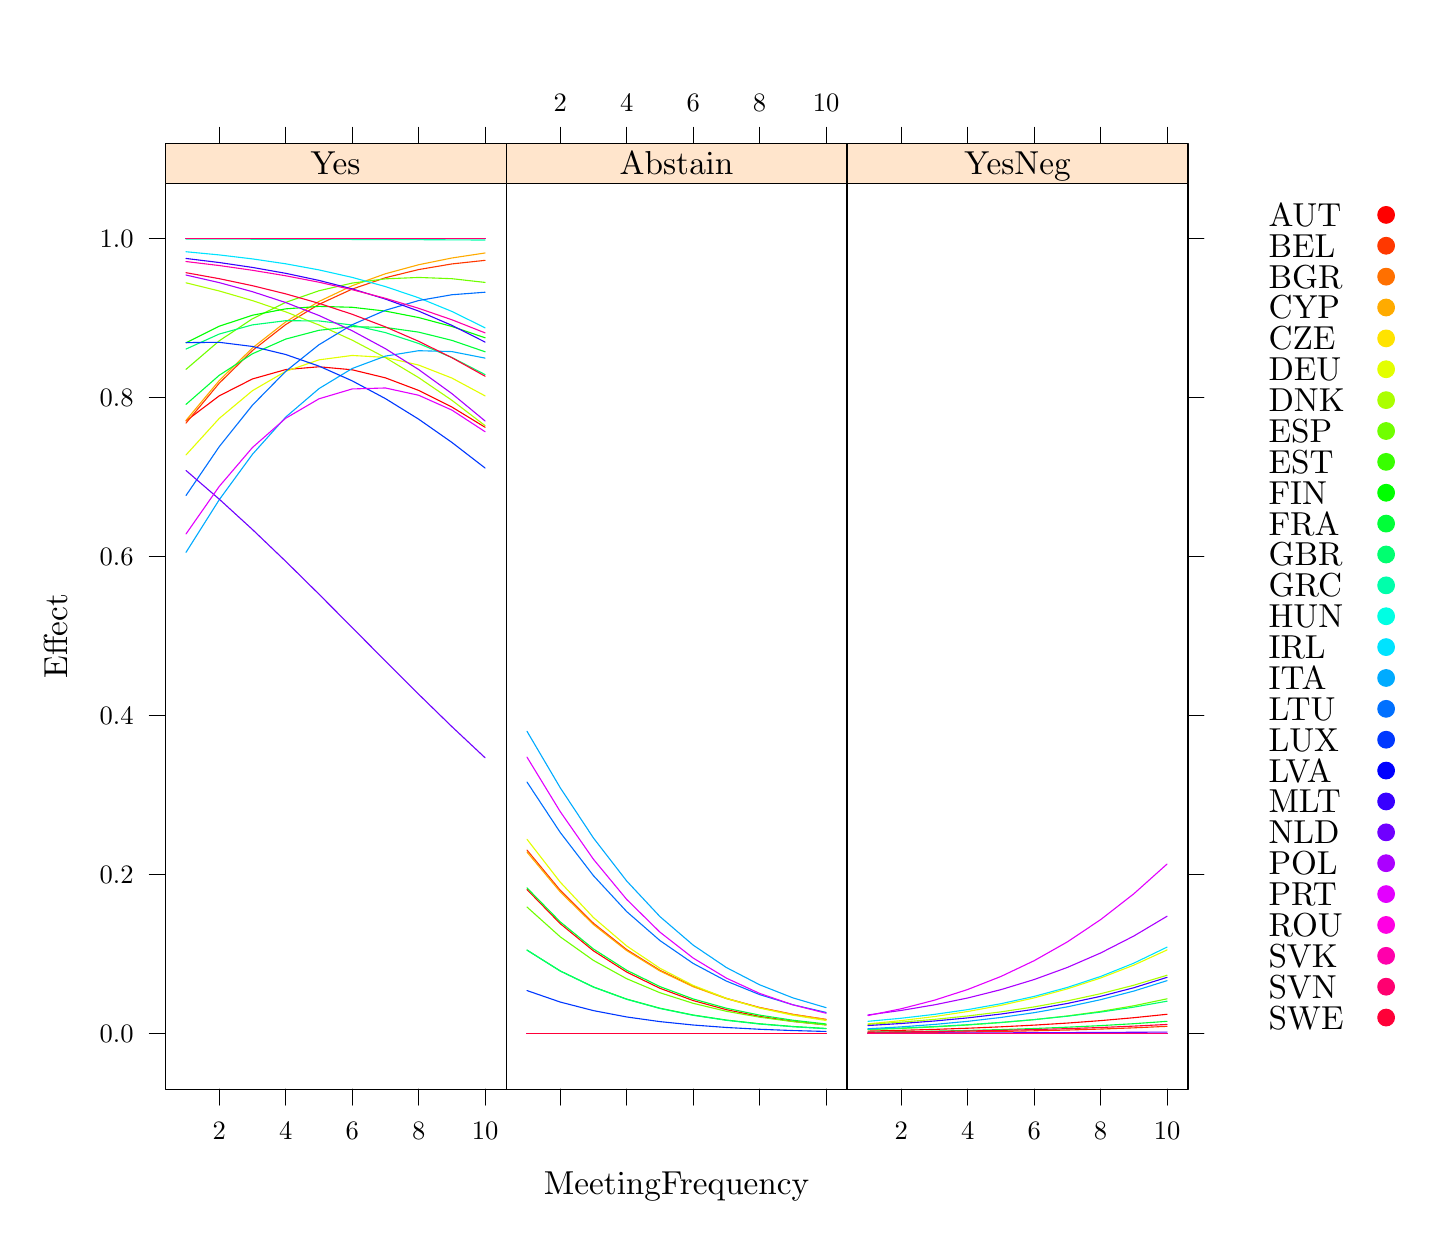
\begin{tikzpicture}[x=1pt,y=1pt]
\definecolor[named]{drawColor}{rgb}{0.00,0.00,0.00}
\definecolor[named]{fillColor}{rgb}{1.00,1.00,1.00}
\fill[color=fillColor,] (0,0) rectangle (505.89,433.62);
\begin{scope}
\path[clip] (  0.00,  0.00) rectangle (505.89,433.62);
\definecolor[named]{fillColor}{rgb}{0.00,0.00,0.00}
\end{scope}
\begin{scope}
\path[clip] (  0.00,  0.00) rectangle (505.89,433.62);
\definecolor[named]{fillColor}{rgb}{0.00,0.00,0.00}

\draw[fill opacity=0.00,draw opacity=0.00,] (  0.00,  0.00) rectangle (505.89,433.62);
\end{scope}
\begin{scope}
\path[clip] (  0.00,  0.00) rectangle (505.89,433.62);
\definecolor[named]{fillColor}{rgb}{0.00,0.00,0.00}
\end{scope}
\begin{scope}
\path[clip] (  0.00,  0.00) rectangle (505.89,433.62);
\definecolor[named]{fillColor}{rgb}{0.00,0.00,0.00}
\definecolor[named]{drawColor}{rgb}{0.00,0.00,0.00}

\node[color=drawColor,anchor=base,inner sep=0pt, outer sep=0pt, scale=  1.20] at (234.47, 12.04) {MeetingFrequency%
};
\end{scope}
\begin{scope}
\path[clip] (  0.00,  0.00) rectangle (505.89,433.62);
\definecolor[named]{fillColor}{rgb}{0.00,0.00,0.00}
\definecolor[named]{drawColor}{rgb}{0.00,0.00,0.00}

\node[rotate= 90.00,color=drawColor,anchor=base,inner sep=0pt, outer sep=0pt, scale=  1.20] at ( 14.29,213.72) {Effect%
};
\end{scope}
\begin{scope}
\path[clip] (  0.00,  0.00) rectangle (505.89,433.62);
\definecolor[named]{fillColor}{rgb}{0.00,0.00,0.00}
\end{scope}
\begin{scope}
\path[clip] (  0.00,  0.00) rectangle (505.89,433.62);
\definecolor[named]{fillColor}{rgb}{0.00,0.00,0.00}
\end{scope}
\begin{scope}
\path[clip] (  0.00,  0.00) rectangle (505.89,433.62);
\definecolor[named]{fillColor}{rgb}{0.00,0.00,0.00}
\end{scope}
\begin{scope}
\path[clip] ( 49.65, 50.02) rectangle (172.86,377.42);
\definecolor[named]{fillColor}{rgb}{0.00,0.00,0.00}
\end{scope}
\begin{scope}
\path[clip] (  0.00,  0.00) rectangle (505.89,433.62);
\definecolor[named]{fillColor}{rgb}{0.00,0.00,0.00}
\end{scope}
\begin{scope}
\path[clip] (  0.00,  0.00) rectangle (505.89,433.62);
\definecolor[named]{fillColor}{rgb}{0.00,0.00,0.00}
\definecolor[named]{drawColor}{rgb}{0.00,0.00,0.00}

\draw[color=drawColor,line cap=round,line join=round,fill opacity=0.00,] ( 69.22,391.87) -- ( 69.22,397.56);

\draw[color=drawColor,line cap=round,line join=round,fill opacity=0.00,] ( 93.24,391.87) -- ( 93.24,397.56);

\draw[color=drawColor,line cap=round,line join=round,fill opacity=0.00,] (117.26,391.87) -- (117.26,397.56);

\draw[color=drawColor,line cap=round,line join=round,fill opacity=0.00,] (141.28,391.87) -- (141.28,397.56);

\draw[color=drawColor,line cap=round,line join=round,fill opacity=0.00,] (165.29,391.87) -- (165.29,397.56);
\end{scope}
\begin{scope}
\path[clip] (  0.00,  0.00) rectangle (505.89,433.62);
\definecolor[named]{fillColor}{rgb}{0.00,0.00,0.00}
\end{scope}
\begin{scope}
\path[clip] (  0.00,  0.00) rectangle (505.89,433.62);
\definecolor[named]{fillColor}{rgb}{0.00,0.00,0.00}
\definecolor[named]{drawColor}{rgb}{0.00,0.00,0.00}

\draw[color=drawColor,line cap=round,line join=round,fill opacity=0.00,] ( 49.65, 70.12) -- ( 43.95, 70.12);

\draw[color=drawColor,line cap=round,line join=round,fill opacity=0.00,] ( 49.65,127.56) -- ( 43.95,127.56);

\draw[color=drawColor,line cap=round,line join=round,fill opacity=0.00,] ( 49.65,185.00) -- ( 43.95,185.00);

\draw[color=drawColor,line cap=round,line join=round,fill opacity=0.00,] ( 49.65,242.43) -- ( 43.95,242.43);

\draw[color=drawColor,line cap=round,line join=round,fill opacity=0.00,] ( 49.65,299.87) -- ( 43.95,299.87);

\draw[color=drawColor,line cap=round,line join=round,fill opacity=0.00,] ( 49.65,357.31) -- ( 43.95,357.31);

\node[color=drawColor,anchor=base east,inner sep=0pt, outer sep=0pt, scale=  0.96] at ( 38.26, 66.81) {0.0%
};

\node[color=drawColor,anchor=base east,inner sep=0pt, outer sep=0pt, scale=  0.96] at ( 38.26,124.25) {0.2%
};

\node[color=drawColor,anchor=base east,inner sep=0pt, outer sep=0pt, scale=  0.96] at ( 38.26,181.69) {0.4%
};

\node[color=drawColor,anchor=base east,inner sep=0pt, outer sep=0pt, scale=  0.96] at ( 38.26,239.13) {0.6%
};

\node[color=drawColor,anchor=base east,inner sep=0pt, outer sep=0pt, scale=  0.96] at ( 38.26,296.57) {0.8%
};

\node[color=drawColor,anchor=base east,inner sep=0pt, outer sep=0pt, scale=  0.96] at ( 38.26,354.01) {1.0%
};
\end{scope}
\begin{scope}
\path[clip] (  0.00,  0.00) rectangle (505.89,433.62);
\definecolor[named]{fillColor}{rgb}{0.00,0.00,0.00}
\end{scope}
\begin{scope}
\path[clip] (  0.00,  0.00) rectangle (505.89,433.62);
\definecolor[named]{fillColor}{rgb}{0.00,0.00,0.00}
\definecolor[named]{drawColor}{rgb}{0.00,0.00,0.00}

\draw[color=drawColor,line cap=round,line join=round,fill opacity=0.00,] ( 69.22, 50.02) -- ( 69.22, 44.32);

\draw[color=drawColor,line cap=round,line join=round,fill opacity=0.00,] ( 93.24, 50.02) -- ( 93.24, 44.32);

\draw[color=drawColor,line cap=round,line join=round,fill opacity=0.00,] (117.26, 50.02) -- (117.26, 44.32);

\draw[color=drawColor,line cap=round,line join=round,fill opacity=0.00,] (141.28, 50.02) -- (141.28, 44.32);

\draw[color=drawColor,line cap=round,line join=round,fill opacity=0.00,] (165.29, 50.02) -- (165.29, 44.32);

\node[color=drawColor,anchor=base,inner sep=0pt, outer sep=0pt, scale=  0.96] at ( 69.22, 32.02) {2%
};

\node[color=drawColor,anchor=base,inner sep=0pt, outer sep=0pt, scale=  0.96] at ( 93.24, 32.02) {4%
};

\node[color=drawColor,anchor=base,inner sep=0pt, outer sep=0pt, scale=  0.96] at (117.26, 32.02) {6%
};

\node[color=drawColor,anchor=base,inner sep=0pt, outer sep=0pt, scale=  0.96] at (141.28, 32.02) {8%
};

\node[color=drawColor,anchor=base,inner sep=0pt, outer sep=0pt, scale=  0.96] at (165.29, 32.02) {10%
};
\end{scope}
\begin{scope}
\path[clip] (  0.00,  0.00) rectangle (505.89,433.62);
\definecolor[named]{fillColor}{rgb}{0.00,0.00,0.00}
\end{scope}
\begin{scope}
\path[clip] ( 49.65, 50.02) rectangle (172.86,377.42);
\definecolor[named]{fillColor}{rgb}{0.00,0.00,0.00}
\definecolor[named]{drawColor}{rgb}{1.00,0.00,0.00}

\draw[color=drawColor,line cap=round,line join=round,fill opacity=0.00,] ( 57.21,291.51) --
	( 69.22,300.58) --
	( 81.23,306.68) --
	( 93.24,310.07) --
	(105.25,311.08) --
	(117.26,309.99) --
	(129.27,307.08) --
	(141.28,302.54) --
	(153.28,296.54) --
	(165.29,289.22);
\definecolor[named]{drawColor}{rgb}{1.00,0.22,0.00}

\draw[color=drawColor,line cap=round,line join=round,fill opacity=0.00,] ( 57.21,290.72) --
	( 69.22,305.15) --
	( 81.23,316.95) --
	( 93.24,326.34) --
	(105.25,333.63) --
	(117.26,339.16) --
	(129.27,343.26) --
	(141.28,346.21) --
	(153.28,348.24) --
	(165.29,349.54);
\definecolor[named]{drawColor}{rgb}{1.00,0.44,0.00}

\draw[color=drawColor,line cap=round,line join=round,fill opacity=0.00,] ( 57.21,357.31) --
	( 69.22,357.31) --
	( 81.23,357.31) --
	( 93.24,357.31) --
	(105.25,357.31) --
	(117.26,357.31) --
	(129.27,357.31) --
	(141.28,357.31) --
	(153.28,357.31) --
	(165.29,357.31);
\definecolor[named]{drawColor}{rgb}{1.00,0.67,0.00}

\draw[color=drawColor,line cap=round,line join=round,fill opacity=0.00,] ( 57.21,291.71) --
	( 69.22,306.09) --
	( 81.23,317.89) --
	( 93.24,327.31) --
	(105.25,334.68) --
	(117.26,340.37) --
	(129.27,344.69) --
	(141.28,347.95) --
	(153.28,350.39) --
	(165.29,352.20);
\definecolor[named]{drawColor}{rgb}{1.00,0.89,0.00}

\draw[color=drawColor,line cap=round,line join=round,fill opacity=0.00,] ( 57.21,357.31) --
	( 69.22,357.31) --
	( 81.23,357.31) --
	( 93.24,357.31) --
	(105.25,357.31) --
	(117.26,357.31) --
	(129.27,357.31) --
	(141.28,357.31) --
	(153.28,357.31) --
	(165.29,357.31);
\definecolor[named]{drawColor}{rgb}{0.89,1.00,0.00}

\draw[color=drawColor,line cap=round,line join=round,fill opacity=0.00,] ( 57.21,279.22) --
	( 69.22,292.42) --
	( 81.23,302.45) --
	( 93.24,309.43) --
	(105.25,313.58) --
	(117.26,315.17) --
	(129.27,314.47) --
	(141.28,311.70) --
	(153.28,307.01) --
	(165.29,300.56);
\definecolor[named]{drawColor}{rgb}{0.67,1.00,0.00}

\draw[color=drawColor,line cap=round,line join=round,fill opacity=0.00,] ( 57.21,341.42) --
	( 69.22,338.47) --
	( 81.23,334.99) --
	( 93.24,330.93) --
	(105.25,326.19) --
	(117.26,320.70) --
	(129.27,314.38) --
	(141.28,307.16) --
	(153.28,298.98) --
	(165.29,289.81);
\definecolor[named]{drawColor}{rgb}{0.44,1.00,0.00}

\draw[color=drawColor,line cap=round,line join=round,fill opacity=0.00,] ( 57.21,310.14) --
	( 69.22,320.46) --
	( 81.23,328.43) --
	( 93.24,334.35) --
	(105.25,338.55) --
	(117.26,341.32) --
	(129.27,342.86) --
	(141.28,343.36) --
	(153.28,342.91) --
	(165.29,341.56);
\definecolor[named]{drawColor}{rgb}{0.22,1.00,0.00}

\draw[color=drawColor,line cap=round,line join=round,fill opacity=0.00,] ( 57.21,357.31) --
	( 69.22,357.31) --
	( 81.23,357.31) --
	( 93.24,357.31) --
	(105.25,357.31) --
	(117.26,357.31) --
	(129.27,357.31) --
	(141.28,357.31) --
	(153.28,357.31) --
	(165.29,357.31);
\definecolor[named]{drawColor}{rgb}{0.00,1.00,0.00}

\draw[color=drawColor,line cap=round,line join=round,fill opacity=0.00,] ( 57.21,319.76) --
	( 69.22,325.73) --
	( 81.23,329.71) --
	( 93.24,332.01) --
	(105.25,332.90) --
	(117.26,332.58) --
	(129.27,331.20) --
	(141.28,328.87) --
	(153.28,325.65) --
	(165.29,321.56);
\definecolor[named]{drawColor}{rgb}{0.00,1.00,0.22}

\draw[color=drawColor,line cap=round,line join=round,fill opacity=0.00,] ( 57.21,297.48) --
	( 69.22,308.00) --
	( 81.23,315.78) --
	( 93.24,321.09) --
	(105.25,324.26) --
	(117.26,325.58) --
	(129.27,325.29) --
	(141.28,323.60) --
	(153.28,320.63) --
	(165.29,316.50);
\definecolor[named]{drawColor}{rgb}{0.00,1.00,0.44}

\draw[color=drawColor,line cap=round,line join=round,fill opacity=0.00,] ( 57.21,317.48) --
	( 69.22,322.91) --
	( 81.23,326.23) --
	( 93.24,327.73) --
	(105.25,327.65) --
	(117.26,326.17) --
	(129.27,323.43) --
	(141.28,319.50) --
	(153.28,314.44) --
	(165.29,308.26);
\definecolor[named]{drawColor}{rgb}{0.00,1.00,0.67}

\draw[color=drawColor,line cap=round,line join=round,fill opacity=0.00,] ( 57.21,357.22) --
	( 69.22,357.20) --
	( 81.23,357.18) --
	( 93.24,357.16) --
	(105.25,357.13) --
	(117.26,357.09) --
	(129.27,357.05) --
	(141.28,357.01) --
	(153.28,356.95) --
	(165.29,356.88);
\definecolor[named]{drawColor}{rgb}{0.00,1.00,0.89}

\draw[color=drawColor,line cap=round,line join=round,fill opacity=0.00,] ( 57.21,357.31) --
	( 69.22,357.31) --
	( 81.23,357.31) --
	( 93.24,357.31) --
	(105.25,357.31) --
	(117.26,357.31) --
	(129.27,357.31) --
	(141.28,357.31) --
	(153.28,357.31) --
	(165.29,357.31);
\definecolor[named]{drawColor}{rgb}{0.00,0.89,1.00}

\draw[color=drawColor,line cap=round,line join=round,fill opacity=0.00,] ( 57.21,352.65) --
	( 69.22,351.50) --
	( 81.23,350.06) --
	( 93.24,348.29) --
	(105.25,346.09) --
	(117.26,343.38) --
	(129.27,340.06) --
	(141.28,336.00) --
	(153.28,331.08) --
	(165.29,325.16);
\definecolor[named]{drawColor}{rgb}{0.00,0.67,1.00}

\draw[color=drawColor,line cap=round,line join=round,fill opacity=0.00,] ( 57.21,244.02) --
	( 69.22,263.03) --
	( 81.23,279.46) --
	( 93.24,292.89) --
	(105.25,303.18) --
	(117.26,310.46) --
	(129.27,314.94) --
	(141.28,316.89) --
	(153.28,316.57) --
	(165.29,314.21);
\definecolor[named]{drawColor}{rgb}{0.00,0.44,1.00}

\draw[color=drawColor,line cap=round,line join=round,fill opacity=0.00,] ( 57.21,264.55) --
	( 69.22,282.21) --
	( 81.23,297.21) --
	( 93.24,309.44) --
	(105.25,319.04) --
	(117.26,326.28) --
	(129.27,331.50) --
	(141.28,335.01) --
	(153.28,337.11) --
	(165.29,338.02);
\definecolor[named]{drawColor}{rgb}{0.00,0.22,1.00}

\draw[color=drawColor,line cap=round,line join=round,fill opacity=0.00,] ( 57.21,319.81) --
	( 69.22,319.92) --
	( 81.23,318.42) --
	( 93.24,315.51) --
	(105.25,311.33) --
	(117.26,306.00) --
	(129.27,299.58) --
	(141.28,292.15) --
	(153.28,283.76) --
	(165.29,274.49);
\definecolor[named]{drawColor}{rgb}{0.00,0.00,1.00}

\draw[color=drawColor,line cap=round,line join=round,fill opacity=0.00,] ( 57.21,357.31) --
	( 69.22,357.31) --
	( 81.23,357.31) --
	( 93.24,357.31) --
	(105.25,357.31) --
	(117.26,357.31) --
	(129.27,357.31) --
	(141.28,357.31) --
	(153.28,357.31) --
	(165.29,357.31);
\definecolor[named]{drawColor}{rgb}{0.22,0.00,1.00}

\draw[color=drawColor,line cap=round,line join=round,fill opacity=0.00,] ( 57.21,350.22) --
	( 69.22,348.75) --
	( 81.23,346.98) --
	( 93.24,344.85) --
	(105.25,342.29) --
	(117.26,339.22) --
	(129.27,335.55) --
	(141.28,331.20) --
	(153.28,326.05) --
	(165.29,320.01);
\definecolor[named]{drawColor}{rgb}{0.44,0.00,1.00}

\draw[color=drawColor,line cap=round,line join=round,fill opacity=0.00,] ( 57.21,273.61) --
	( 69.22,263.25) --
	( 81.23,252.27) --
	( 93.24,240.78) --
	(105.25,228.93) --
	(117.26,216.85) --
	(129.27,204.74) --
	(141.28,192.75) --
	(153.28,181.05) --
	(165.29,169.79);
\definecolor[named]{drawColor}{rgb}{0.67,0.00,1.00}

\draw[color=drawColor,line cap=round,line join=round,fill opacity=0.00,] ( 57.21,344.23) --
	( 69.22,341.49) --
	( 81.23,338.21) --
	( 93.24,334.29) --
	(105.25,329.62) --
	(117.26,324.10) --
	(129.27,317.62) --
	(141.28,310.08) --
	(153.28,301.39) --
	(165.29,291.49);
\definecolor[named]{drawColor}{rgb}{0.89,0.00,1.00}

\draw[color=drawColor,line cap=round,line join=round,fill opacity=0.00,] ( 57.21,250.66) --
	( 69.22,267.85) --
	( 81.23,281.91) --
	( 93.24,292.48) --
	(105.25,299.50) --
	(117.26,303.07) --
	(129.27,303.42) --
	(141.28,300.79) --
	(153.28,295.44) --
	(165.29,287.61);
\definecolor[named]{drawColor}{rgb}{1.00,0.00,0.89}

\draw[color=drawColor,line cap=round,line join=round,fill opacity=0.00,] ( 57.21,357.31) --
	( 69.22,357.31) --
	( 81.23,357.31) --
	( 93.24,357.31) --
	(105.25,357.31) --
	(117.26,357.31) --
	(129.27,357.31) --
	(141.28,357.31) --
	(153.28,357.31) --
	(165.29,357.31);
\definecolor[named]{drawColor}{rgb}{1.00,0.00,0.67}

\draw[color=drawColor,line cap=round,line join=round,fill opacity=0.00,] ( 57.21,349.11) --
	( 69.22,347.66) --
	( 81.23,345.95) --
	( 93.24,343.96) --
	(105.25,341.64) --
	(117.26,338.94) --
	(129.27,335.82) --
	(141.28,332.21) --
	(153.28,328.07) --
	(165.29,323.33);
\definecolor[named]{drawColor}{rgb}{1.00,0.00,0.44}

\draw[color=drawColor,line cap=round,line join=round,fill opacity=0.00,] ( 57.21,357.31) --
	( 69.22,357.31) --
	( 81.23,357.31) --
	( 93.24,357.31) --
	(105.25,357.31) --
	(117.26,357.31) --
	(129.27,357.31) --
	(141.28,357.31) --
	(153.28,357.31) --
	(165.29,357.31);
\definecolor[named]{drawColor}{rgb}{1.00,0.00,0.22}

\draw[color=drawColor,line cap=round,line join=round,fill opacity=0.00,] ( 57.21,345.08) --
	( 69.22,342.91) --
	( 81.23,340.38) --
	( 93.24,337.43) --
	(105.25,334.01) --
	(117.26,330.05) --
	(129.27,325.50) --
	(141.28,320.29) --
	(153.28,314.37) --
	(165.29,307.67);
\end{scope}
\begin{scope}
\path[clip] (  0.00,  0.00) rectangle (505.89,433.62);
\definecolor[named]{fillColor}{rgb}{0.00,0.00,0.00}
\end{scope}
\begin{scope}
\path[clip] (  0.00,  0.00) rectangle (505.89,433.62);
\definecolor[named]{fillColor}{rgb}{0.00,0.00,0.00}
\definecolor[named]{drawColor}{rgb}{0.00,0.00,0.00}

\draw[color=drawColor,line cap=round,line join=round,fill opacity=0.00,] ( 49.65, 50.02) rectangle (172.86,377.42);
\end{scope}
\begin{scope}
\path[clip] (  0.00,  0.00) rectangle (505.89,433.62);
\definecolor[named]{fillColor}{rgb}{0.00,0.00,0.00}
\end{scope}
\begin{scope}
\path[clip] (  0.00,  0.00) rectangle (505.89,433.62);
\definecolor[named]{fillColor}{rgb}{0.00,0.00,0.00}
\end{scope}
\begin{scope}
\path[clip] ( 49.65,377.42) rectangle (172.86,391.87);
\definecolor[named]{fillColor}{rgb}{0.00,0.00,0.00}
\definecolor[named]{drawColor}{rgb}{1.00,0.90,0.80}
\definecolor[named]{fillColor}{rgb}{1.00,0.90,0.80}

\draw[color=drawColor,line cap=round,line join=round,fill=fillColor,] ( 49.65,377.42) rectangle (172.86,391.87);
\definecolor[named]{drawColor}{rgb}{0.00,0.00,0.00}

\node[color=drawColor,anchor=base west,inner sep=0pt, outer sep=0pt, scale=  1.20] at (102.22,380.51) {Yes%
};
\end{scope}
\begin{scope}
\path[clip] (  0.00,  0.00) rectangle (505.89,433.62);
\definecolor[named]{fillColor}{rgb}{0.00,0.00,0.00}
\end{scope}
\begin{scope}
\path[clip] (  0.00,  0.00) rectangle (505.89,433.62);
\definecolor[named]{fillColor}{rgb}{0.00,0.00,0.00}
\definecolor[named]{drawColor}{rgb}{0.00,0.00,0.00}

\draw[color=drawColor,line cap=round,line join=round,fill opacity=0.00,] ( 49.65,377.42) rectangle (172.86,391.87);
\end{scope}
\begin{scope}
\path[clip] (  0.00,  0.00) rectangle (505.89,433.62);
\definecolor[named]{fillColor}{rgb}{0.00,0.00,0.00}
\end{scope}
\begin{scope}
\path[clip] (  0.00,  0.00) rectangle (505.89,433.62);
\definecolor[named]{fillColor}{rgb}{0.00,0.00,0.00}
\end{scope}
\begin{scope}
\path[clip] (172.86, 50.02) rectangle (296.07,377.42);
\definecolor[named]{fillColor}{rgb}{0.00,0.00,0.00}
\end{scope}
\begin{scope}
\path[clip] (  0.00,  0.00) rectangle (505.89,433.62);
\definecolor[named]{fillColor}{rgb}{0.00,0.00,0.00}
\end{scope}
\begin{scope}
\path[clip] (  0.00,  0.00) rectangle (505.89,433.62);
\definecolor[named]{fillColor}{rgb}{0.00,0.00,0.00}
\definecolor[named]{drawColor}{rgb}{0.00,0.00,0.00}

\draw[color=drawColor,line cap=round,line join=round,fill opacity=0.00,] (192.43,391.87) -- (192.43,397.56);

\draw[color=drawColor,line cap=round,line join=round,fill opacity=0.00,] (216.45,391.87) -- (216.45,397.56);

\draw[color=drawColor,line cap=round,line join=round,fill opacity=0.00,] (240.47,391.87) -- (240.47,397.56);

\draw[color=drawColor,line cap=round,line join=round,fill opacity=0.00,] (264.49,391.87) -- (264.49,397.56);

\draw[color=drawColor,line cap=round,line join=round,fill opacity=0.00,] (288.51,391.87) -- (288.51,397.56);

\node[color=drawColor,anchor=base,inner sep=0pt, outer sep=0pt, scale=  0.96] at (192.43,403.25) {2%
};

\node[color=drawColor,anchor=base,inner sep=0pt, outer sep=0pt, scale=  0.96] at (216.45,403.25) {4%
};

\node[color=drawColor,anchor=base,inner sep=0pt, outer sep=0pt, scale=  0.96] at (240.47,403.25) {6%
};

\node[color=drawColor,anchor=base,inner sep=0pt, outer sep=0pt, scale=  0.96] at (264.49,403.25) {8%
};

\node[color=drawColor,anchor=base,inner sep=0pt, outer sep=0pt, scale=  0.96] at (288.51,403.25) {10%
};
\end{scope}
\begin{scope}
\path[clip] (  0.00,  0.00) rectangle (505.89,433.62);
\definecolor[named]{fillColor}{rgb}{0.00,0.00,0.00}
\end{scope}
\begin{scope}
\path[clip] (  0.00,  0.00) rectangle (505.89,433.62);
\definecolor[named]{fillColor}{rgb}{0.00,0.00,0.00}
\end{scope}
\begin{scope}
\path[clip] (  0.00,  0.00) rectangle (505.89,433.62);
\definecolor[named]{fillColor}{rgb}{0.00,0.00,0.00}
\end{scope}
\begin{scope}
\path[clip] (  0.00,  0.00) rectangle (505.89,433.62);
\definecolor[named]{fillColor}{rgb}{0.00,0.00,0.00}
\definecolor[named]{drawColor}{rgb}{0.00,0.00,0.00}

\draw[color=drawColor,line cap=round,line join=round,fill opacity=0.00,] (192.43, 50.02) -- (192.43, 44.32);

\draw[color=drawColor,line cap=round,line join=round,fill opacity=0.00,] (216.45, 50.02) -- (216.45, 44.32);

\draw[color=drawColor,line cap=round,line join=round,fill opacity=0.00,] (240.47, 50.02) -- (240.47, 44.32);

\draw[color=drawColor,line cap=round,line join=round,fill opacity=0.00,] (264.49, 50.02) -- (264.49, 44.32);

\draw[color=drawColor,line cap=round,line join=round,fill opacity=0.00,] (288.51, 50.02) -- (288.51, 44.32);
\end{scope}
\begin{scope}
\path[clip] (  0.00,  0.00) rectangle (505.89,433.62);
\definecolor[named]{fillColor}{rgb}{0.00,0.00,0.00}
\end{scope}
\begin{scope}
\path[clip] (172.86, 50.02) rectangle (296.07,377.42);
\definecolor[named]{fillColor}{rgb}{0.00,0.00,0.00}
\definecolor[named]{drawColor}{rgb}{1.00,0.00,0.00}

\draw[color=drawColor,line cap=round,line join=round,fill opacity=0.00,] (180.42,122.20) --
	(192.43,109.87) --
	(204.44,100.03) --
	(216.45, 92.36) --
	(228.46, 86.50) --
	(240.47, 82.07) --
	(252.48, 78.77) --
	(264.49, 76.34) --
	(276.50, 74.56) --
	(288.51, 73.27);
\definecolor[named]{drawColor}{rgb}{1.00,0.22,0.00}

\draw[color=drawColor,line cap=round,line join=round,fill opacity=0.00,] (180.42,136.45) --
	(192.43,121.93) --
	(204.44,110.01) --
	(216.45,100.48) --
	(228.46, 93.01) --
	(240.47, 87.25) --
	(252.48, 82.87) --
	(264.49, 79.57) --
	(276.50, 77.10) --
	(288.51, 75.26);
\definecolor[named]{drawColor}{rgb}{1.00,0.44,0.00}

\draw[color=drawColor,line cap=round,line join=round,fill opacity=0.00,] (180.42, 70.12) --
	(192.43, 70.12) --
	(204.44, 70.12) --
	(216.45, 70.12) --
	(228.46, 70.12) --
	(240.47, 70.12) --
	(252.48, 70.12) --
	(264.49, 70.12) --
	(276.50, 70.12) --
	(288.51, 70.12);
\definecolor[named]{drawColor}{rgb}{1.00,0.67,0.00}

\draw[color=drawColor,line cap=round,line join=round,fill opacity=0.00,] (180.42,135.72) --
	(192.43,121.34) --
	(204.44,109.54) --
	(216.45,100.12) --
	(228.46, 92.75) --
	(240.47, 87.06) --
	(252.48, 82.74) --
	(264.49, 79.48) --
	(276.50, 77.04) --
	(288.51, 75.23);
\definecolor[named]{drawColor}{rgb}{1.00,0.89,0.00}

\draw[color=drawColor,line cap=round,line join=round,fill opacity=0.00,] (180.42, 70.12) --
	(192.43, 70.12) --
	(204.44, 70.12) --
	(216.45, 70.12) --
	(228.46, 70.12) --
	(240.47, 70.12) --
	(252.48, 70.12) --
	(264.49, 70.12) --
	(276.50, 70.12) --
	(288.51, 70.12);
\definecolor[named]{drawColor}{rgb}{0.89,1.00,0.00}

\draw[color=drawColor,line cap=round,line join=round,fill opacity=0.00,] (180.42,140.36) --
	(192.43,124.87) --
	(204.44,112.07) --
	(216.45,101.80) --
	(228.46, 93.75) --
	(240.47, 87.55) --
	(252.48, 82.87) --
	(264.49, 79.36) --
	(276.50, 76.76) --
	(288.51, 74.86);
\definecolor[named]{drawColor}{rgb}{0.67,1.00,0.00}

\draw[color=drawColor,line cap=round,line join=round,fill opacity=0.00,] (180.42, 70.12) --
	(192.43, 70.12) --
	(204.44, 70.12) --
	(216.45, 70.12) --
	(228.46, 70.12) --
	(240.47, 70.12) --
	(252.48, 70.12) --
	(264.49, 70.12) --
	(276.50, 70.12) --
	(288.51, 70.12);
\definecolor[named]{drawColor}{rgb}{0.44,1.00,0.00}

\draw[color=drawColor,line cap=round,line join=round,fill opacity=0.00,] (180.42,115.87) --
	(192.43,105.10) --
	(204.44, 96.58) --
	(216.45, 89.96) --
	(228.46, 84.90) --
	(240.47, 81.07) --
	(252.48, 78.19) --
	(264.49, 76.05) --
	(276.50, 74.46) --
	(288.51, 73.28);
\definecolor[named]{drawColor}{rgb}{0.22,1.00,0.00}

\draw[color=drawColor,line cap=round,line join=round,fill opacity=0.00,] (180.42, 70.12) --
	(192.43, 70.12) --
	(204.44, 70.12) --
	(216.45, 70.12) --
	(228.46, 70.12) --
	(240.47, 70.12) --
	(252.48, 70.12) --
	(264.49, 70.12) --
	(276.50, 70.12) --
	(288.51, 70.12);
\definecolor[named]{drawColor}{rgb}{0.00,1.00,0.00}

\draw[color=drawColor,line cap=round,line join=round,fill opacity=0.00,] (180.42,100.30) --
	(192.43, 92.78) --
	(204.44, 86.99) --
	(216.45, 82.60) --
	(228.46, 79.30) --
	(240.47, 76.84) --
	(252.48, 75.02) --
	(264.49, 73.68) --
	(276.50, 72.70) --
	(288.51, 71.98);
\definecolor[named]{drawColor}{rgb}{0.00,1.00,0.22}

\draw[color=drawColor,line cap=round,line join=round,fill opacity=0.00,] (180.42,122.78) --
	(192.43,110.51) --
	(204.44,100.70) --
	(216.45, 93.02) --
	(228.46, 87.12) --
	(240.47, 82.65) --
	(252.48, 79.30) --
	(264.49, 76.80) --
	(276.50, 74.96) --
	(288.51, 73.61);
\definecolor[named]{drawColor}{rgb}{0.00,1.00,0.44}

\draw[color=drawColor,line cap=round,line join=round,fill opacity=0.00,] (180.42,100.31) --
	(192.43, 92.74) --
	(204.44, 86.92) --
	(216.45, 82.51) --
	(228.46, 79.20) --
	(240.47, 76.74) --
	(252.48, 74.92) --
	(264.49, 73.58) --
	(276.50, 72.61) --
	(288.51, 71.90);
\definecolor[named]{drawColor}{rgb}{0.00,1.00,0.67}

\draw[color=drawColor,line cap=round,line join=round,fill opacity=0.00,] (180.42, 70.12) --
	(192.43, 70.12) --
	(204.44, 70.12) --
	(216.45, 70.12) --
	(228.46, 70.12) --
	(240.47, 70.12) --
	(252.48, 70.12) --
	(264.49, 70.12) --
	(276.50, 70.12) --
	(288.51, 70.12);
\definecolor[named]{drawColor}{rgb}{0.00,1.00,0.89}

\draw[color=drawColor,line cap=round,line join=round,fill opacity=0.00,] (180.42, 70.12) --
	(192.43, 70.12) --
	(204.44, 70.12) --
	(216.45, 70.12) --
	(228.46, 70.12) --
	(240.47, 70.12) --
	(252.48, 70.12) --
	(264.49, 70.12) --
	(276.50, 70.12) --
	(288.51, 70.12);
\definecolor[named]{drawColor}{rgb}{0.00,0.89,1.00}

\draw[color=drawColor,line cap=round,line join=round,fill opacity=0.00,] (180.42, 70.12) --
	(192.43, 70.12) --
	(204.44, 70.12) --
	(216.45, 70.12) --
	(228.46, 70.12) --
	(240.47, 70.12) --
	(252.48, 70.12) --
	(264.49, 70.12) --
	(276.50, 70.12) --
	(288.51, 70.12);
\definecolor[named]{drawColor}{rgb}{0.00,0.67,1.00}

\draw[color=drawColor,line cap=round,line join=round,fill opacity=0.00,] (180.42,179.38) --
	(192.43,158.98) --
	(204.44,140.81) --
	(216.45,125.27) --
	(228.46,112.42) --
	(240.47,102.10) --
	(252.48, 94.00) --
	(264.49, 87.77) --
	(276.50, 83.04) --
	(288.51, 79.50);
\definecolor[named]{drawColor}{rgb}{0.00,0.44,1.00}

\draw[color=drawColor,line cap=round,line join=round,fill opacity=0.00,] (180.42,161.04) --
	(192.43,142.83) --
	(204.44,127.20) --
	(216.45,114.22) --
	(228.46,103.75) --
	(240.47, 95.49) --
	(252.48, 89.10) --
	(264.49, 84.22) --
	(276.50, 80.54) --
	(288.51, 77.78);
\definecolor[named]{drawColor}{rgb}{0.00,0.22,1.00}

\draw[color=drawColor,line cap=round,line join=round,fill opacity=0.00,] (180.42, 85.68) --
	(192.43, 81.53) --
	(204.44, 78.43) --
	(216.45, 76.14) --
	(228.46, 74.46) --
	(240.47, 73.23) --
	(252.48, 72.34) --
	(264.49, 71.69) --
	(276.50, 71.23) --
	(288.51, 70.90);
\definecolor[named]{drawColor}{rgb}{0.00,0.00,1.00}

\draw[color=drawColor,line cap=round,line join=round,fill opacity=0.00,] (180.42, 70.12) --
	(192.43, 70.12) --
	(204.44, 70.12) --
	(216.45, 70.12) --
	(228.46, 70.12) --
	(240.47, 70.12) --
	(252.48, 70.12) --
	(264.49, 70.12) --
	(276.50, 70.12) --
	(288.51, 70.12);
\definecolor[named]{drawColor}{rgb}{0.22,0.00,1.00}

\draw[color=drawColor,line cap=round,line join=round,fill opacity=0.00,] (180.42, 70.12) --
	(192.43, 70.12) --
	(204.44, 70.12) --
	(216.45, 70.12) --
	(228.46, 70.12) --
	(240.47, 70.12) --
	(252.48, 70.12) --
	(264.49, 70.12) --
	(276.50, 70.12) --
	(288.51, 70.12);
\definecolor[named]{drawColor}{rgb}{0.44,0.00,1.00}

\draw[color=drawColor,line cap=round,line join=round,fill opacity=0.00,] (180.42, 70.12) --
	(192.43, 70.12) --
	(204.44, 70.12) --
	(216.45, 70.12) --
	(228.46, 70.12) --
	(240.47, 70.12) --
	(252.48, 70.12) --
	(264.49, 70.12) --
	(276.50, 70.12) --
	(288.51, 70.12);
\definecolor[named]{drawColor}{rgb}{0.67,0.00,1.00}

\draw[color=drawColor,line cap=round,line join=round,fill opacity=0.00,] (180.42, 70.12) --
	(192.43, 70.12) --
	(204.44, 70.12) --
	(216.45, 70.12) --
	(228.46, 70.12) --
	(240.47, 70.12) --
	(252.48, 70.12) --
	(264.49, 70.12) --
	(276.50, 70.12) --
	(288.51, 70.12);
\definecolor[named]{drawColor}{rgb}{0.89,0.00,1.00}

\draw[color=drawColor,line cap=round,line join=round,fill opacity=0.00,] (180.42,170.04) --
	(192.43,150.35) --
	(204.44,133.12) --
	(216.45,118.61) --
	(228.46,106.79) --
	(240.47, 97.43) --
	(252.48, 90.17) --
	(264.49, 84.65) --
	(276.50, 80.53) --
	(288.51, 77.48);
\definecolor[named]{drawColor}{rgb}{1.00,0.00,0.89}

\draw[color=drawColor,line cap=round,line join=round,fill opacity=0.00,] (180.42, 70.12) --
	(192.43, 70.12) --
	(204.44, 70.12) --
	(216.45, 70.12) --
	(228.46, 70.12) --
	(240.47, 70.12) --
	(252.48, 70.12) --
	(264.49, 70.12) --
	(276.50, 70.12) --
	(288.51, 70.12);
\definecolor[named]{drawColor}{rgb}{1.00,0.00,0.67}

\draw[color=drawColor,line cap=round,line join=round,fill opacity=0.00,] (180.42, 70.12) --
	(192.43, 70.12) --
	(204.44, 70.12) --
	(216.45, 70.12) --
	(228.46, 70.12) --
	(240.47, 70.12) --
	(252.48, 70.12) --
	(264.49, 70.12) --
	(276.50, 70.12) --
	(288.51, 70.12);
\definecolor[named]{drawColor}{rgb}{1.00,0.00,0.44}

\draw[color=drawColor,line cap=round,line join=round,fill opacity=0.00,] (180.42, 70.12) --
	(192.43, 70.12) --
	(204.44, 70.12) --
	(216.45, 70.12) --
	(228.46, 70.12) --
	(240.47, 70.12) --
	(252.48, 70.12) --
	(264.49, 70.12) --
	(276.50, 70.12) --
	(288.51, 70.12);
\definecolor[named]{drawColor}{rgb}{1.00,0.00,0.22}

\draw[color=drawColor,line cap=round,line join=round,fill opacity=0.00,] (180.42, 70.12) --
	(192.43, 70.12) --
	(204.44, 70.12) --
	(216.45, 70.12) --
	(228.46, 70.12) --
	(240.47, 70.12) --
	(252.48, 70.12) --
	(264.49, 70.12) --
	(276.50, 70.12) --
	(288.51, 70.12);
\end{scope}
\begin{scope}
\path[clip] (  0.00,  0.00) rectangle (505.89,433.62);
\definecolor[named]{fillColor}{rgb}{0.00,0.00,0.00}
\end{scope}
\begin{scope}
\path[clip] (  0.00,  0.00) rectangle (505.89,433.62);
\definecolor[named]{fillColor}{rgb}{0.00,0.00,0.00}
\definecolor[named]{drawColor}{rgb}{0.00,0.00,0.00}

\draw[color=drawColor,line cap=round,line join=round,fill opacity=0.00,] (172.86, 50.02) rectangle (296.07,377.42);
\end{scope}
\begin{scope}
\path[clip] (  0.00,  0.00) rectangle (505.89,433.62);
\definecolor[named]{fillColor}{rgb}{0.00,0.00,0.00}
\end{scope}
\begin{scope}
\path[clip] (  0.00,  0.00) rectangle (505.89,433.62);
\definecolor[named]{fillColor}{rgb}{0.00,0.00,0.00}
\end{scope}
\begin{scope}
\path[clip] (172.86,377.42) rectangle (296.07,391.87);
\definecolor[named]{fillColor}{rgb}{0.00,0.00,0.00}
\definecolor[named]{drawColor}{rgb}{1.00,0.90,0.80}
\definecolor[named]{fillColor}{rgb}{1.00,0.90,0.80}

\draw[color=drawColor,line cap=round,line join=round,fill=fillColor,] (172.86,377.42) rectangle (296.07,391.87);
\definecolor[named]{drawColor}{rgb}{0.00,0.00,0.00}

\node[color=drawColor,anchor=base west,inner sep=0pt, outer sep=0pt, scale=  1.20] at (213.94,380.51) {Abstain%
};
\end{scope}
\begin{scope}
\path[clip] (  0.00,  0.00) rectangle (505.89,433.62);
\definecolor[named]{fillColor}{rgb}{0.00,0.00,0.00}
\end{scope}
\begin{scope}
\path[clip] (  0.00,  0.00) rectangle (505.89,433.62);
\definecolor[named]{fillColor}{rgb}{0.00,0.00,0.00}
\definecolor[named]{drawColor}{rgb}{0.00,0.00,0.00}

\draw[color=drawColor,line cap=round,line join=round,fill opacity=0.00,] (172.86,377.42) rectangle (296.07,391.87);
\end{scope}
\begin{scope}
\path[clip] (  0.00,  0.00) rectangle (505.89,433.62);
\definecolor[named]{fillColor}{rgb}{0.00,0.00,0.00}
\end{scope}
\begin{scope}
\path[clip] (  0.00,  0.00) rectangle (505.89,433.62);
\definecolor[named]{fillColor}{rgb}{0.00,0.00,0.00}
\end{scope}
\begin{scope}
\path[clip] (296.07, 50.02) rectangle (419.29,377.42);
\definecolor[named]{fillColor}{rgb}{0.00,0.00,0.00}
\end{scope}
\begin{scope}
\path[clip] (  0.00,  0.00) rectangle (505.89,433.62);
\definecolor[named]{fillColor}{rgb}{0.00,0.00,0.00}
\end{scope}
\begin{scope}
\path[clip] (  0.00,  0.00) rectangle (505.89,433.62);
\definecolor[named]{fillColor}{rgb}{0.00,0.00,0.00}
\definecolor[named]{drawColor}{rgb}{0.00,0.00,0.00}

\draw[color=drawColor,line cap=round,line join=round,fill opacity=0.00,] (315.65,391.87) -- (315.65,397.56);

\draw[color=drawColor,line cap=round,line join=round,fill opacity=0.00,] (339.67,391.87) -- (339.67,397.56);

\draw[color=drawColor,line cap=round,line join=round,fill opacity=0.00,] (363.69,391.87) -- (363.69,397.56);

\draw[color=drawColor,line cap=round,line join=round,fill opacity=0.00,] (387.70,391.87) -- (387.70,397.56);

\draw[color=drawColor,line cap=round,line join=round,fill opacity=0.00,] (411.72,391.87) -- (411.72,397.56);
\end{scope}
\begin{scope}
\path[clip] (  0.00,  0.00) rectangle (505.89,433.62);
\definecolor[named]{fillColor}{rgb}{0.00,0.00,0.00}
\end{scope}
\begin{scope}
\path[clip] (  0.00,  0.00) rectangle (505.89,433.62);
\definecolor[named]{fillColor}{rgb}{0.00,0.00,0.00}
\end{scope}
\begin{scope}
\path[clip] (  0.00,  0.00) rectangle (505.89,433.62);
\definecolor[named]{fillColor}{rgb}{0.00,0.00,0.00}
\end{scope}
\begin{scope}
\path[clip] (  0.00,  0.00) rectangle (505.89,433.62);
\definecolor[named]{fillColor}{rgb}{0.00,0.00,0.00}
\definecolor[named]{drawColor}{rgb}{0.00,0.00,0.00}

\draw[color=drawColor,line cap=round,line join=round,fill opacity=0.00,] (315.65, 50.02) -- (315.65, 44.32);

\draw[color=drawColor,line cap=round,line join=round,fill opacity=0.00,] (339.67, 50.02) -- (339.67, 44.32);

\draw[color=drawColor,line cap=round,line join=round,fill opacity=0.00,] (363.69, 50.02) -- (363.69, 44.32);

\draw[color=drawColor,line cap=round,line join=round,fill opacity=0.00,] (387.70, 50.02) -- (387.70, 44.32);

\draw[color=drawColor,line cap=round,line join=round,fill opacity=0.00,] (411.72, 50.02) -- (411.72, 44.32);

\node[color=drawColor,anchor=base,inner sep=0pt, outer sep=0pt, scale=  0.96] at (315.65, 32.02) {2%
};

\node[color=drawColor,anchor=base,inner sep=0pt, outer sep=0pt, scale=  0.96] at (339.67, 32.02) {4%
};

\node[color=drawColor,anchor=base,inner sep=0pt, outer sep=0pt, scale=  0.96] at (363.69, 32.02) {6%
};

\node[color=drawColor,anchor=base,inner sep=0pt, outer sep=0pt, scale=  0.96] at (387.70, 32.02) {8%
};

\node[color=drawColor,anchor=base,inner sep=0pt, outer sep=0pt, scale=  0.96] at (411.72, 32.02) {10%
};

\draw[color=drawColor,line cap=round,line join=round,fill opacity=0.00,] (419.29, 70.12) -- (424.98, 70.12);

\draw[color=drawColor,line cap=round,line join=round,fill opacity=0.00,] (419.29,127.56) -- (424.98,127.56);

\draw[color=drawColor,line cap=round,line join=round,fill opacity=0.00,] (419.29,185.00) -- (424.98,185.00);

\draw[color=drawColor,line cap=round,line join=round,fill opacity=0.00,] (419.29,242.43) -- (424.98,242.43);

\draw[color=drawColor,line cap=round,line join=round,fill opacity=0.00,] (419.29,299.87) -- (424.98,299.87);

\draw[color=drawColor,line cap=round,line join=round,fill opacity=0.00,] (419.29,357.31) -- (424.98,357.31);
\end{scope}
\begin{scope}
\path[clip] (  0.00,  0.00) rectangle (505.89,433.62);
\definecolor[named]{fillColor}{rgb}{0.00,0.00,0.00}
\end{scope}
\begin{scope}
\path[clip] (296.07, 50.02) rectangle (419.29,377.42);
\definecolor[named]{fillColor}{rgb}{0.00,0.00,0.00}
\definecolor[named]{drawColor}{rgb}{1.00,0.00,0.00}

\draw[color=drawColor,line cap=round,line join=round,fill opacity=0.00,] (303.64, 71.03) --
	(315.65, 71.31) --
	(327.66, 71.65) --
	(339.67, 72.07) --
	(351.68, 72.58) --
	(363.69, 73.19) --
	(375.69, 73.93) --
	(387.70, 74.82) --
	(399.71, 75.87) --
	(411.72, 77.11);
\definecolor[named]{drawColor}{rgb}{1.00,0.22,0.00}

\draw[color=drawColor,line cap=round,line join=round,fill opacity=0.00,] (303.64, 70.39) --
	(315.65, 70.48) --
	(327.66, 70.59) --
	(339.67, 70.73) --
	(351.68, 70.91) --
	(363.69, 71.14) --
	(375.69, 71.42) --
	(387.70, 71.77) --
	(399.71, 72.21) --
	(411.72, 72.75);
\definecolor[named]{drawColor}{rgb}{1.00,0.44,0.00}

\draw[color=drawColor,line cap=round,line join=round,fill opacity=0.00,] (303.64, 70.12) --
	(315.65, 70.12) --
	(327.66, 70.12) --
	(339.67, 70.12) --
	(351.68, 70.12) --
	(363.69, 70.12) --
	(375.69, 70.12) --
	(387.70, 70.12) --
	(399.71, 70.12) --
	(411.72, 70.12);
\definecolor[named]{drawColor}{rgb}{1.00,0.67,0.00}

\draw[color=drawColor,line cap=round,line join=round,fill opacity=0.00,] (303.64, 70.12) --
	(315.65, 70.12) --
	(327.66, 70.12) --
	(339.67, 70.12) --
	(351.68, 70.12) --
	(363.69, 70.12) --
	(375.69, 70.12) --
	(387.70, 70.12) --
	(399.71, 70.12) --
	(411.72, 70.12);
\definecolor[named]{drawColor}{rgb}{1.00,0.89,0.00}

\draw[color=drawColor,line cap=round,line join=round,fill opacity=0.00,] (303.64, 70.12) --
	(315.65, 70.12) --
	(327.66, 70.12) --
	(339.67, 70.12) --
	(351.68, 70.12) --
	(363.69, 70.12) --
	(375.69, 70.12) --
	(387.70, 70.12) --
	(399.71, 70.12) --
	(411.72, 70.12);
\definecolor[named]{drawColor}{rgb}{0.89,1.00,0.00}

\draw[color=drawColor,line cap=round,line join=round,fill opacity=0.00,] (303.64, 73.64) --
	(315.65, 74.82) --
	(327.66, 76.29) --
	(339.67, 78.11) --
	(351.68, 80.33) --
	(363.69, 83.03) --
	(375.69, 86.30) --
	(387.70, 90.21) --
	(399.71, 94.87) --
	(411.72,100.36);
\definecolor[named]{drawColor}{rgb}{0.67,1.00,0.00}

\draw[color=drawColor,line cap=round,line join=round,fill opacity=0.00,] (303.64, 73.46) --
	(315.65, 74.27) --
	(327.66, 75.27) --
	(339.67, 76.49) --
	(351.68, 77.98) --
	(363.69, 79.78) --
	(375.69, 81.95) --
	(387.70, 84.54) --
	(399.71, 87.61) --
	(411.72, 91.22);
\definecolor[named]{drawColor}{rgb}{0.44,1.00,0.00}

\draw[color=drawColor,line cap=round,line join=round,fill opacity=0.00,] (303.64, 71.55) --
	(315.65, 71.99) --
	(327.66, 72.54) --
	(339.67, 73.23) --
	(351.68, 74.10) --
	(363.69, 75.17) --
	(375.69, 76.50) --
	(387.70, 78.14) --
	(399.71, 80.18) --
	(411.72, 82.70);
\definecolor[named]{drawColor}{rgb}{0.22,1.00,0.00}

\draw[color=drawColor,line cap=round,line join=round,fill opacity=0.00,] (303.64, 70.12) --
	(315.65, 70.12) --
	(327.66, 70.12) --
	(339.67, 70.12) --
	(351.68, 70.12) --
	(363.69, 70.12) --
	(375.69, 70.12) --
	(387.70, 70.12) --
	(399.71, 70.12) --
	(411.72, 70.12);
\definecolor[named]{drawColor}{rgb}{0.00,1.00,0.00}

\draw[color=drawColor,line cap=round,line join=round,fill opacity=0.00,] (303.64, 70.12) --
	(315.65, 70.12) --
	(327.66, 70.12) --
	(339.67, 70.12) --
	(351.68, 70.12) --
	(363.69, 70.12) --
	(375.69, 70.12) --
	(387.70, 70.12) --
	(399.71, 70.12) --
	(411.72, 70.12);
\definecolor[named]{drawColor}{rgb}{0.00,1.00,0.22}

\draw[color=drawColor,line cap=round,line join=round,fill opacity=0.00,] (303.64, 70.64) --
	(315.65, 70.81) --
	(327.66, 71.01) --
	(339.67, 71.27) --
	(351.68, 71.58) --
	(363.69, 71.97) --
	(375.69, 72.44) --
	(387.70, 73.01) --
	(399.71, 73.71) --
	(411.72, 74.56);
\definecolor[named]{drawColor}{rgb}{0.00,1.00,0.44}

\draw[color=drawColor,line cap=round,line join=round,fill opacity=0.00,] (303.64, 71.68) --
	(315.65, 72.12) --
	(327.66, 72.67) --
	(339.67, 73.34) --
	(351.68, 74.17) --
	(363.69, 75.18) --
	(375.69, 76.41) --
	(387.70, 77.90) --
	(399.71, 79.69) --
	(411.72, 81.84);
\definecolor[named]{drawColor}{rgb}{0.00,1.00,0.67}

\draw[color=drawColor,line cap=round,line join=round,fill opacity=0.00,] (303.64, 70.12) --
	(315.65, 70.12) --
	(327.66, 70.12) --
	(339.67, 70.12) --
	(351.68, 70.12) --
	(363.69, 70.12) --
	(375.69, 70.12) --
	(387.70, 70.12) --
	(399.71, 70.12) --
	(411.72, 70.12);
\definecolor[named]{drawColor}{rgb}{0.00,1.00,0.89}

\draw[color=drawColor,line cap=round,line join=round,fill opacity=0.00,] (303.64, 70.12) --
	(315.65, 70.12) --
	(327.66, 70.12) --
	(339.67, 70.12) --
	(351.68, 70.12) --
	(363.69, 70.12) --
	(375.69, 70.12) --
	(387.70, 70.12) --
	(399.71, 70.12) --
	(411.72, 70.12);
\definecolor[named]{drawColor}{rgb}{0.00,0.89,1.00}

\draw[color=drawColor,line cap=round,line join=round,fill opacity=0.00,] (303.64, 74.56) --
	(315.65, 75.68) --
	(327.66, 77.07) --
	(339.67, 78.79) --
	(351.68, 80.93) --
	(363.69, 83.57) --
	(375.69, 86.81) --
	(387.70, 90.77) --
	(399.71, 95.58) --
	(411.72,101.38);
\definecolor[named]{drawColor}{rgb}{0.00,0.67,1.00}

\draw[color=drawColor,line cap=round,line join=round,fill opacity=0.00,] (303.64, 71.87) --
	(315.65, 72.56) --
	(327.66, 73.44) --
	(339.67, 74.56) --
	(351.68, 75.96) --
	(363.69, 77.69) --
	(375.69, 79.80) --
	(387.70, 82.38) --
	(399.71, 85.50) --
	(411.72, 89.26);
\definecolor[named]{drawColor}{rgb}{0.00,0.44,1.00}

\draw[color=drawColor,line cap=round,line join=round,fill opacity=0.00,] (303.64, 70.12) --
	(315.65, 70.12) --
	(327.66, 70.12) --
	(339.67, 70.12) --
	(351.68, 70.12) --
	(363.69, 70.12) --
	(375.69, 70.12) --
	(387.70, 70.12) --
	(399.71, 70.12) --
	(411.72, 70.12);
\definecolor[named]{drawColor}{rgb}{0.00,0.22,1.00}

\draw[color=drawColor,line cap=round,line join=round,fill opacity=0.00,] (303.64, 70.12) --
	(315.65, 70.12) --
	(327.66, 70.12) --
	(339.67, 70.12) --
	(351.68, 70.12) --
	(363.69, 70.12) --
	(375.69, 70.12) --
	(387.70, 70.12) --
	(399.71, 70.12) --
	(411.72, 70.12);
\definecolor[named]{drawColor}{rgb}{0.00,0.00,1.00}

\draw[color=drawColor,line cap=round,line join=round,fill opacity=0.00,] (303.64, 70.12) --
	(315.65, 70.12) --
	(327.66, 70.12) --
	(339.67, 70.12) --
	(351.68, 70.12) --
	(363.69, 70.12) --
	(375.69, 70.12) --
	(387.70, 70.12) --
	(399.71, 70.12) --
	(411.72, 70.12);
\definecolor[named]{drawColor}{rgb}{0.22,0.00,1.00}

\draw[color=drawColor,line cap=round,line join=round,fill opacity=0.00,] (303.64, 73.04) --
	(315.65, 73.78) --
	(327.66, 74.68) --
	(339.67, 75.81) --
	(351.68, 77.20) --
	(363.69, 78.91) --
	(375.69, 81.02) --
	(387.70, 83.59) --
	(399.71, 86.70) --
	(411.72, 90.46);
\definecolor[named]{drawColor}{rgb}{0.44,0.00,1.00}

\draw[color=drawColor,line cap=round,line join=round,fill opacity=0.00,] (303.64, 70.26) --
	(315.65, 70.29) --
	(327.66, 70.32) --
	(339.67, 70.36) --
	(351.68, 70.40) --
	(363.69, 70.44) --
	(375.69, 70.49) --
	(387.70, 70.55) --
	(399.71, 70.61) --
	(411.72, 70.67);
\definecolor[named]{drawColor}{rgb}{0.67,0.00,1.00}

\draw[color=drawColor,line cap=round,line join=round,fill opacity=0.00,] (303.64, 76.86) --
	(315.65, 78.50) --
	(327.66, 80.52) --
	(339.67, 83.00) --
	(351.68, 86.01) --
	(363.69, 89.66) --
	(375.69, 94.04) --
	(387.70, 99.25) --
	(399.71,105.39) --
	(411.72,112.54);
\definecolor[named]{drawColor}{rgb}{0.89,0.00,1.00}

\draw[color=drawColor,line cap=round,line join=round,fill opacity=0.00,] (303.64, 76.65) --
	(315.65, 79.10) --
	(327.66, 82.20) --
	(339.67, 86.06) --
	(351.68, 90.77) --
	(363.69, 96.47) --
	(375.69,103.27) --
	(387.70,111.30) --
	(399.71,120.65) --
	(411.72,131.40);
\definecolor[named]{drawColor}{rgb}{1.00,0.00,0.89}

\draw[color=drawColor,line cap=round,line join=round,fill opacity=0.00,] (303.64, 70.12) --
	(315.65, 70.12) --
	(327.66, 70.12) --
	(339.67, 70.12) --
	(351.68, 70.12) --
	(363.69, 70.12) --
	(375.69, 70.12) --
	(387.70, 70.12) --
	(399.71, 70.12) --
	(411.72, 70.12);
\definecolor[named]{drawColor}{rgb}{1.00,0.00,0.67}

\draw[color=drawColor,line cap=round,line join=round,fill opacity=0.00,] (303.64, 70.12) --
	(315.65, 70.12) --
	(327.66, 70.12) --
	(339.67, 70.12) --
	(351.68, 70.12) --
	(363.69, 70.12) --
	(375.69, 70.12) --
	(387.70, 70.12) --
	(399.71, 70.12) --
	(411.72, 70.12);
\definecolor[named]{drawColor}{rgb}{1.00,0.00,0.44}

\draw[color=drawColor,line cap=round,line join=round,fill opacity=0.00,] (303.64, 70.12) --
	(315.65, 70.12) --
	(327.66, 70.12) --
	(339.67, 70.12) --
	(351.68, 70.12) --
	(363.69, 70.12) --
	(375.69, 70.12) --
	(387.70, 70.12) --
	(399.71, 70.12) --
	(411.72, 70.12);
\definecolor[named]{drawColor}{rgb}{1.00,0.00,0.22}

\draw[color=drawColor,line cap=round,line join=round,fill opacity=0.00,] (303.64, 70.61) --
	(315.65, 70.73) --
	(327.66, 70.88) --
	(339.67, 71.07) --
	(351.68, 71.30) --
	(363.69, 71.58) --
	(375.69, 71.92) --
	(387.70, 72.33) --
	(399.71, 72.83) --
	(411.72, 73.43);
\end{scope}
\begin{scope}
\path[clip] (  0.00,  0.00) rectangle (505.89,433.62);
\definecolor[named]{fillColor}{rgb}{0.00,0.00,0.00}
\end{scope}
\begin{scope}
\path[clip] (  0.00,  0.00) rectangle (505.89,433.62);
\definecolor[named]{fillColor}{rgb}{0.00,0.00,0.00}
\definecolor[named]{drawColor}{rgb}{0.00,0.00,0.00}

\draw[color=drawColor,line cap=round,line join=round,fill opacity=0.00,] (296.07, 50.02) rectangle (419.29,377.42);
\end{scope}
\begin{scope}
\path[clip] (  0.00,  0.00) rectangle (505.89,433.62);
\definecolor[named]{fillColor}{rgb}{0.00,0.00,0.00}
\end{scope}
\begin{scope}
\path[clip] (  0.00,  0.00) rectangle (505.89,433.62);
\definecolor[named]{fillColor}{rgb}{0.00,0.00,0.00}
\end{scope}
\begin{scope}
\path[clip] (296.07,377.42) rectangle (419.29,391.87);
\definecolor[named]{fillColor}{rgb}{0.00,0.00,0.00}
\definecolor[named]{drawColor}{rgb}{1.00,0.90,0.80}
\definecolor[named]{fillColor}{rgb}{1.00,0.90,0.80}

\draw[color=drawColor,line cap=round,line join=round,fill=fillColor,] (296.07,377.42) rectangle (419.29,391.87);
\definecolor[named]{drawColor}{rgb}{0.00,0.00,0.00}

\node[color=drawColor,anchor=base west,inner sep=0pt, outer sep=0pt, scale=  1.20] at (338.49,380.51) {YesNeg%
};
\end{scope}
\begin{scope}
\path[clip] (  0.00,  0.00) rectangle (505.89,433.62);
\definecolor[named]{fillColor}{rgb}{0.00,0.00,0.00}
\end{scope}
\begin{scope}
\path[clip] (  0.00,  0.00) rectangle (505.89,433.62);
\definecolor[named]{fillColor}{rgb}{0.00,0.00,0.00}
\definecolor[named]{drawColor}{rgb}{0.00,0.00,0.00}

\draw[color=drawColor,line cap=round,line join=round,fill opacity=0.00,] (296.07,377.42) rectangle (419.29,391.87);
\end{scope}
\begin{scope}
\path[clip] (  0.00,  0.00) rectangle (505.89,433.62);
\definecolor[named]{fillColor}{rgb}{0.00,0.00,0.00}
\end{scope}
\begin{scope}
\path[clip] (  0.00,  0.00) rectangle (505.89,433.62);
\definecolor[named]{fillColor}{rgb}{0.00,0.00,0.00}

\draw[fill opacity=0.00,draw opacity=0.00,] (442.38, 70.34) rectangle (499.87,371.54);
\end{scope}
\begin{scope}
\path[clip] (  0.00,  0.00) rectangle (505.89,433.62);
\definecolor[named]{fillColor}{rgb}{0.00,0.00,0.00}
\definecolor[named]{drawColor}{rgb}{0.00,0.00,0.00}

\node[color=drawColor,anchor=base west,inner sep=0pt, outer sep=0pt, scale=  1.20] at (448.38,361.83) {AUT%
};
\end{scope}
\begin{scope}
\path[clip] (  0.00,  0.00) rectangle (505.89,433.62);
\definecolor[named]{fillColor}{rgb}{0.00,0.00,0.00}
\definecolor[named]{drawColor}{rgb}{0.00,0.00,0.00}

\node[color=drawColor,anchor=base west,inner sep=0pt, outer sep=0pt, scale=  1.20] at (448.38,350.68) {BEL%
};
\end{scope}
\begin{scope}
\path[clip] (  0.00,  0.00) rectangle (505.89,433.62);
\definecolor[named]{fillColor}{rgb}{0.00,0.00,0.00}
\definecolor[named]{drawColor}{rgb}{0.00,0.00,0.00}

\node[color=drawColor,anchor=base west,inner sep=0pt, outer sep=0pt, scale=  1.20] at (448.38,339.52) {BGR%
};
\end{scope}
\begin{scope}
\path[clip] (  0.00,  0.00) rectangle (505.89,433.62);
\definecolor[named]{fillColor}{rgb}{0.00,0.00,0.00}
\definecolor[named]{drawColor}{rgb}{0.00,0.00,0.00}

\node[color=drawColor,anchor=base west,inner sep=0pt, outer sep=0pt, scale=  1.20] at (448.38,328.36) {CYP%
};
\end{scope}
\begin{scope}
\path[clip] (  0.00,  0.00) rectangle (505.89,433.62);
\definecolor[named]{fillColor}{rgb}{0.00,0.00,0.00}
\definecolor[named]{drawColor}{rgb}{0.00,0.00,0.00}

\node[color=drawColor,anchor=base west,inner sep=0pt, outer sep=0pt, scale=  1.20] at (448.38,317.21) {CZE%
};
\end{scope}
\begin{scope}
\path[clip] (  0.00,  0.00) rectangle (505.89,433.62);
\definecolor[named]{fillColor}{rgb}{0.00,0.00,0.00}
\definecolor[named]{drawColor}{rgb}{0.00,0.00,0.00}

\node[color=drawColor,anchor=base west,inner sep=0pt, outer sep=0pt, scale=  1.20] at (448.38,306.05) {DEU%
};
\end{scope}
\begin{scope}
\path[clip] (  0.00,  0.00) rectangle (505.89,433.62);
\definecolor[named]{fillColor}{rgb}{0.00,0.00,0.00}
\definecolor[named]{drawColor}{rgb}{0.00,0.00,0.00}

\node[color=drawColor,anchor=base west,inner sep=0pt, outer sep=0pt, scale=  1.20] at (448.38,294.90) {DNK%
};
\end{scope}
\begin{scope}
\path[clip] (  0.00,  0.00) rectangle (505.89,433.62);
\definecolor[named]{fillColor}{rgb}{0.00,0.00,0.00}
\definecolor[named]{drawColor}{rgb}{0.00,0.00,0.00}

\node[color=drawColor,anchor=base west,inner sep=0pt, outer sep=0pt, scale=  1.20] at (448.38,283.74) {ESP%
};
\end{scope}
\begin{scope}
\path[clip] (  0.00,  0.00) rectangle (505.89,433.62);
\definecolor[named]{fillColor}{rgb}{0.00,0.00,0.00}
\definecolor[named]{drawColor}{rgb}{0.00,0.00,0.00}

\node[color=drawColor,anchor=base west,inner sep=0pt, outer sep=0pt, scale=  1.20] at (448.38,272.59) {EST%
};
\end{scope}
\begin{scope}
\path[clip] (  0.00,  0.00) rectangle (505.89,433.62);
\definecolor[named]{fillColor}{rgb}{0.00,0.00,0.00}
\definecolor[named]{drawColor}{rgb}{0.00,0.00,0.00}

\node[color=drawColor,anchor=base west,inner sep=0pt, outer sep=0pt, scale=  1.20] at (448.38,261.43) {FIN%
};
\end{scope}
\begin{scope}
\path[clip] (  0.00,  0.00) rectangle (505.89,433.62);
\definecolor[named]{fillColor}{rgb}{0.00,0.00,0.00}
\definecolor[named]{drawColor}{rgb}{0.00,0.00,0.00}

\node[color=drawColor,anchor=base west,inner sep=0pt, outer sep=0pt, scale=  1.20] at (448.38,250.28) {FRA%
};
\end{scope}
\begin{scope}
\path[clip] (  0.00,  0.00) rectangle (505.89,433.62);
\definecolor[named]{fillColor}{rgb}{0.00,0.00,0.00}
\definecolor[named]{drawColor}{rgb}{0.00,0.00,0.00}

\node[color=drawColor,anchor=base west,inner sep=0pt, outer sep=0pt, scale=  1.20] at (448.38,239.12) {GBR%
};
\end{scope}
\begin{scope}
\path[clip] (  0.00,  0.00) rectangle (505.89,433.62);
\definecolor[named]{fillColor}{rgb}{0.00,0.00,0.00}
\definecolor[named]{drawColor}{rgb}{0.00,0.00,0.00}

\node[color=drawColor,anchor=base west,inner sep=0pt, outer sep=0pt, scale=  1.20] at (448.38,227.97) {GRC%
};
\end{scope}
\begin{scope}
\path[clip] (  0.00,  0.00) rectangle (505.89,433.62);
\definecolor[named]{fillColor}{rgb}{0.00,0.00,0.00}
\definecolor[named]{drawColor}{rgb}{0.00,0.00,0.00}

\node[color=drawColor,anchor=base west,inner sep=0pt, outer sep=0pt, scale=  1.20] at (448.38,216.81) {HUN%
};
\end{scope}
\begin{scope}
\path[clip] (  0.00,  0.00) rectangle (505.89,433.62);
\definecolor[named]{fillColor}{rgb}{0.00,0.00,0.00}
\definecolor[named]{drawColor}{rgb}{0.00,0.00,0.00}

\node[color=drawColor,anchor=base west,inner sep=0pt, outer sep=0pt, scale=  1.20] at (448.38,205.65) {IRL%
};
\end{scope}
\begin{scope}
\path[clip] (  0.00,  0.00) rectangle (505.89,433.62);
\definecolor[named]{fillColor}{rgb}{0.00,0.00,0.00}
\definecolor[named]{drawColor}{rgb}{0.00,0.00,0.00}

\node[color=drawColor,anchor=base west,inner sep=0pt, outer sep=0pt, scale=  1.20] at (448.38,194.50) {ITA%
};
\end{scope}
\begin{scope}
\path[clip] (  0.00,  0.00) rectangle (505.89,433.62);
\definecolor[named]{fillColor}{rgb}{0.00,0.00,0.00}
\definecolor[named]{drawColor}{rgb}{0.00,0.00,0.00}

\node[color=drawColor,anchor=base west,inner sep=0pt, outer sep=0pt, scale=  1.20] at (448.38,183.34) {LTU%
};
\end{scope}
\begin{scope}
\path[clip] (  0.00,  0.00) rectangle (505.89,433.62);
\definecolor[named]{fillColor}{rgb}{0.00,0.00,0.00}
\definecolor[named]{drawColor}{rgb}{0.00,0.00,0.00}

\node[color=drawColor,anchor=base west,inner sep=0pt, outer sep=0pt, scale=  1.20] at (448.38,172.19) {LUX%
};
\end{scope}
\begin{scope}
\path[clip] (  0.00,  0.00) rectangle (505.89,433.62);
\definecolor[named]{fillColor}{rgb}{0.00,0.00,0.00}
\definecolor[named]{drawColor}{rgb}{0.00,0.00,0.00}

\node[color=drawColor,anchor=base west,inner sep=0pt, outer sep=0pt, scale=  1.20] at (448.38,161.03) {LVA%
};
\end{scope}
\begin{scope}
\path[clip] (  0.00,  0.00) rectangle (505.89,433.62);
\definecolor[named]{fillColor}{rgb}{0.00,0.00,0.00}
\definecolor[named]{drawColor}{rgb}{0.00,0.00,0.00}

\node[color=drawColor,anchor=base west,inner sep=0pt, outer sep=0pt, scale=  1.20] at (448.38,149.88) {MLT%
};
\end{scope}
\begin{scope}
\path[clip] (  0.00,  0.00) rectangle (505.89,433.62);
\definecolor[named]{fillColor}{rgb}{0.00,0.00,0.00}
\definecolor[named]{drawColor}{rgb}{0.00,0.00,0.00}

\node[color=drawColor,anchor=base west,inner sep=0pt, outer sep=0pt, scale=  1.20] at (448.38,138.72) {NLD%
};
\end{scope}
\begin{scope}
\path[clip] (  0.00,  0.00) rectangle (505.89,433.62);
\definecolor[named]{fillColor}{rgb}{0.00,0.00,0.00}
\definecolor[named]{drawColor}{rgb}{0.00,0.00,0.00}

\node[color=drawColor,anchor=base west,inner sep=0pt, outer sep=0pt, scale=  1.20] at (448.38,127.57) {POL%
};
\end{scope}
\begin{scope}
\path[clip] (  0.00,  0.00) rectangle (505.89,433.62);
\definecolor[named]{fillColor}{rgb}{0.00,0.00,0.00}
\definecolor[named]{drawColor}{rgb}{0.00,0.00,0.00}

\node[color=drawColor,anchor=base west,inner sep=0pt, outer sep=0pt, scale=  1.20] at (448.38,116.41) {PRT%
};
\end{scope}
\begin{scope}
\path[clip] (  0.00,  0.00) rectangle (505.89,433.62);
\definecolor[named]{fillColor}{rgb}{0.00,0.00,0.00}
\definecolor[named]{drawColor}{rgb}{0.00,0.00,0.00}

\node[color=drawColor,anchor=base west,inner sep=0pt, outer sep=0pt, scale=  1.20] at (448.38,105.26) {ROU%
};
\end{scope}
\begin{scope}
\path[clip] (  0.00,  0.00) rectangle (505.89,433.62);
\definecolor[named]{fillColor}{rgb}{0.00,0.00,0.00}
\definecolor[named]{drawColor}{rgb}{0.00,0.00,0.00}

\node[color=drawColor,anchor=base west,inner sep=0pt, outer sep=0pt, scale=  1.20] at (448.38, 94.10) {SVK%
};
\end{scope}
\begin{scope}
\path[clip] (  0.00,  0.00) rectangle (505.89,433.62);
\definecolor[named]{fillColor}{rgb}{0.00,0.00,0.00}
\definecolor[named]{drawColor}{rgb}{0.00,0.00,0.00}

\node[color=drawColor,anchor=base west,inner sep=0pt, outer sep=0pt, scale=  1.20] at (448.38, 82.94) {SVN%
};
\end{scope}
\begin{scope}
\path[clip] (  0.00,  0.00) rectangle (505.89,433.62);
\definecolor[named]{fillColor}{rgb}{0.00,0.00,0.00}
\definecolor[named]{drawColor}{rgb}{0.00,0.00,0.00}

\node[color=drawColor,anchor=base west,inner sep=0pt, outer sep=0pt, scale=  1.20] at (448.38, 71.79) {SWE%
};
\end{scope}
\begin{scope}
\path[clip] (  0.00,  0.00) rectangle (505.89,433.62);
\definecolor[named]{fillColor}{rgb}{0.00,0.00,0.00}
\definecolor[named]{drawColor}{rgb}{1.00,0.00,0.00}
\definecolor[named]{fillColor}{rgb}{1.00,0.00,0.00}

\draw[color=drawColor,line cap=round,line join=round,fill=fillColor,] (490.87,365.96) circle (  3.01);
\end{scope}
\begin{scope}
\path[clip] (  0.00,  0.00) rectangle (505.89,433.62);
\definecolor[named]{fillColor}{rgb}{0.00,0.00,0.00}
\definecolor[named]{drawColor}{rgb}{1.00,0.22,0.00}
\definecolor[named]{fillColor}{rgb}{1.00,0.22,0.00}

\draw[color=drawColor,line cap=round,line join=round,fill=fillColor,] (490.87,354.81) circle (  3.01);
\end{scope}
\begin{scope}
\path[clip] (  0.00,  0.00) rectangle (505.89,433.62);
\definecolor[named]{fillColor}{rgb}{0.00,0.00,0.00}
\definecolor[named]{drawColor}{rgb}{1.00,0.44,0.00}
\definecolor[named]{fillColor}{rgb}{1.00,0.44,0.00}

\draw[color=drawColor,line cap=round,line join=round,fill=fillColor,] (490.87,343.65) circle (  3.01);
\end{scope}
\begin{scope}
\path[clip] (  0.00,  0.00) rectangle (505.89,433.62);
\definecolor[named]{fillColor}{rgb}{0.00,0.00,0.00}
\definecolor[named]{drawColor}{rgb}{1.00,0.67,0.00}
\definecolor[named]{fillColor}{rgb}{1.00,0.67,0.00}

\draw[color=drawColor,line cap=round,line join=round,fill=fillColor,] (490.87,332.50) circle (  3.01);
\end{scope}
\begin{scope}
\path[clip] (  0.00,  0.00) rectangle (505.89,433.62);
\definecolor[named]{fillColor}{rgb}{0.00,0.00,0.00}
\definecolor[named]{drawColor}{rgb}{1.00,0.89,0.00}
\definecolor[named]{fillColor}{rgb}{1.00,0.89,0.00}

\draw[color=drawColor,line cap=round,line join=round,fill=fillColor,] (490.87,321.34) circle (  3.01);
\end{scope}
\begin{scope}
\path[clip] (  0.00,  0.00) rectangle (505.89,433.62);
\definecolor[named]{fillColor}{rgb}{0.00,0.00,0.00}
\definecolor[named]{drawColor}{rgb}{0.89,1.00,0.00}
\definecolor[named]{fillColor}{rgb}{0.89,1.00,0.00}

\draw[color=drawColor,line cap=round,line join=round,fill=fillColor,] (490.87,310.19) circle (  3.01);
\end{scope}
\begin{scope}
\path[clip] (  0.00,  0.00) rectangle (505.89,433.62);
\definecolor[named]{fillColor}{rgb}{0.00,0.00,0.00}
\definecolor[named]{drawColor}{rgb}{0.67,1.00,0.00}
\definecolor[named]{fillColor}{rgb}{0.67,1.00,0.00}

\draw[color=drawColor,line cap=round,line join=round,fill=fillColor,] (490.87,299.03) circle (  3.01);
\end{scope}
\begin{scope}
\path[clip] (  0.00,  0.00) rectangle (505.89,433.62);
\definecolor[named]{fillColor}{rgb}{0.00,0.00,0.00}
\definecolor[named]{drawColor}{rgb}{0.44,1.00,0.00}
\definecolor[named]{fillColor}{rgb}{0.44,1.00,0.00}

\draw[color=drawColor,line cap=round,line join=round,fill=fillColor,] (490.87,287.87) circle (  3.01);
\end{scope}
\begin{scope}
\path[clip] (  0.00,  0.00) rectangle (505.89,433.62);
\definecolor[named]{fillColor}{rgb}{0.00,0.00,0.00}
\definecolor[named]{drawColor}{rgb}{0.22,1.00,0.00}
\definecolor[named]{fillColor}{rgb}{0.22,1.00,0.00}

\draw[color=drawColor,line cap=round,line join=round,fill=fillColor,] (490.87,276.72) circle (  3.01);
\end{scope}
\begin{scope}
\path[clip] (  0.00,  0.00) rectangle (505.89,433.62);
\definecolor[named]{fillColor}{rgb}{0.00,0.00,0.00}
\definecolor[named]{drawColor}{rgb}{0.00,1.00,0.00}
\definecolor[named]{fillColor}{rgb}{0.00,1.00,0.00}

\draw[color=drawColor,line cap=round,line join=round,fill=fillColor,] (490.87,265.56) circle (  3.01);
\end{scope}
\begin{scope}
\path[clip] (  0.00,  0.00) rectangle (505.89,433.62);
\definecolor[named]{fillColor}{rgb}{0.00,0.00,0.00}
\definecolor[named]{drawColor}{rgb}{0.00,1.00,0.22}
\definecolor[named]{fillColor}{rgb}{0.00,1.00,0.22}

\draw[color=drawColor,line cap=round,line join=round,fill=fillColor,] (490.87,254.41) circle (  3.01);
\end{scope}
\begin{scope}
\path[clip] (  0.00,  0.00) rectangle (505.89,433.62);
\definecolor[named]{fillColor}{rgb}{0.00,0.00,0.00}
\definecolor[named]{drawColor}{rgb}{0.00,1.00,0.44}
\definecolor[named]{fillColor}{rgb}{0.00,1.00,0.44}

\draw[color=drawColor,line cap=round,line join=round,fill=fillColor,] (490.87,243.25) circle (  3.01);
\end{scope}
\begin{scope}
\path[clip] (  0.00,  0.00) rectangle (505.89,433.62);
\definecolor[named]{fillColor}{rgb}{0.00,0.00,0.00}
\definecolor[named]{drawColor}{rgb}{0.00,1.00,0.67}
\definecolor[named]{fillColor}{rgb}{0.00,1.00,0.67}

\draw[color=drawColor,line cap=round,line join=round,fill=fillColor,] (490.87,232.10) circle (  3.01);
\end{scope}
\begin{scope}
\path[clip] (  0.00,  0.00) rectangle (505.89,433.62);
\definecolor[named]{fillColor}{rgb}{0.00,0.00,0.00}
\definecolor[named]{drawColor}{rgb}{0.00,1.00,0.89}
\definecolor[named]{fillColor}{rgb}{0.00,1.00,0.89}

\draw[color=drawColor,line cap=round,line join=round,fill=fillColor,] (490.87,220.94) circle (  3.01);
\end{scope}
\begin{scope}
\path[clip] (  0.00,  0.00) rectangle (505.89,433.62);
\definecolor[named]{fillColor}{rgb}{0.00,0.00,0.00}
\definecolor[named]{drawColor}{rgb}{0.00,0.89,1.00}
\definecolor[named]{fillColor}{rgb}{0.00,0.89,1.00}

\draw[color=drawColor,line cap=round,line join=round,fill=fillColor,] (490.87,209.79) circle (  3.01);
\end{scope}
\begin{scope}
\path[clip] (  0.00,  0.00) rectangle (505.89,433.62);
\definecolor[named]{fillColor}{rgb}{0.00,0.00,0.00}
\definecolor[named]{drawColor}{rgb}{0.00,0.67,1.00}
\definecolor[named]{fillColor}{rgb}{0.00,0.67,1.00}

\draw[color=drawColor,line cap=round,line join=round,fill=fillColor,] (490.87,198.63) circle (  3.01);
\end{scope}
\begin{scope}
\path[clip] (  0.00,  0.00) rectangle (505.89,433.62);
\definecolor[named]{fillColor}{rgb}{0.00,0.00,0.00}
\definecolor[named]{drawColor}{rgb}{0.00,0.44,1.00}
\definecolor[named]{fillColor}{rgb}{0.00,0.44,1.00}

\draw[color=drawColor,line cap=round,line join=round,fill=fillColor,] (490.87,187.48) circle (  3.01);
\end{scope}
\begin{scope}
\path[clip] (  0.00,  0.00) rectangle (505.89,433.62);
\definecolor[named]{fillColor}{rgb}{0.00,0.00,0.00}
\definecolor[named]{drawColor}{rgb}{0.00,0.22,1.00}
\definecolor[named]{fillColor}{rgb}{0.00,0.22,1.00}

\draw[color=drawColor,line cap=round,line join=round,fill=fillColor,] (490.87,176.32) circle (  3.01);
\end{scope}
\begin{scope}
\path[clip] (  0.00,  0.00) rectangle (505.89,433.62);
\definecolor[named]{fillColor}{rgb}{0.00,0.00,0.00}
\definecolor[named]{drawColor}{rgb}{0.00,0.00,1.00}
\definecolor[named]{fillColor}{rgb}{0.00,0.00,1.00}

\draw[color=drawColor,line cap=round,line join=round,fill=fillColor,] (490.87,165.17) circle (  3.01);
\end{scope}
\begin{scope}
\path[clip] (  0.00,  0.00) rectangle (505.89,433.62);
\definecolor[named]{fillColor}{rgb}{0.00,0.00,0.00}
\definecolor[named]{drawColor}{rgb}{0.22,0.00,1.00}
\definecolor[named]{fillColor}{rgb}{0.22,0.00,1.00}

\draw[color=drawColor,line cap=round,line join=round,fill=fillColor,] (490.87,154.01) circle (  3.01);
\end{scope}
\begin{scope}
\path[clip] (  0.00,  0.00) rectangle (505.89,433.62);
\definecolor[named]{fillColor}{rgb}{0.00,0.00,0.00}
\definecolor[named]{drawColor}{rgb}{0.44,0.00,1.00}
\definecolor[named]{fillColor}{rgb}{0.44,0.00,1.00}

\draw[color=drawColor,line cap=round,line join=round,fill=fillColor,] (490.87,142.85) circle (  3.01);
\end{scope}
\begin{scope}
\path[clip] (  0.00,  0.00) rectangle (505.89,433.62);
\definecolor[named]{fillColor}{rgb}{0.00,0.00,0.00}
\definecolor[named]{drawColor}{rgb}{0.67,0.00,1.00}
\definecolor[named]{fillColor}{rgb}{0.67,0.00,1.00}

\draw[color=drawColor,line cap=round,line join=round,fill=fillColor,] (490.87,131.70) circle (  3.01);
\end{scope}
\begin{scope}
\path[clip] (  0.00,  0.00) rectangle (505.89,433.62);
\definecolor[named]{fillColor}{rgb}{0.00,0.00,0.00}
\definecolor[named]{drawColor}{rgb}{0.89,0.00,1.00}
\definecolor[named]{fillColor}{rgb}{0.89,0.00,1.00}

\draw[color=drawColor,line cap=round,line join=round,fill=fillColor,] (490.87,120.54) circle (  3.01);
\end{scope}
\begin{scope}
\path[clip] (  0.00,  0.00) rectangle (505.89,433.62);
\definecolor[named]{fillColor}{rgb}{0.00,0.00,0.00}
\definecolor[named]{drawColor}{rgb}{1.00,0.00,0.89}
\definecolor[named]{fillColor}{rgb}{1.00,0.00,0.89}

\draw[color=drawColor,line cap=round,line join=round,fill=fillColor,] (490.87,109.39) circle (  3.01);
\end{scope}
\begin{scope}
\path[clip] (  0.00,  0.00) rectangle (505.89,433.62);
\definecolor[named]{fillColor}{rgb}{0.00,0.00,0.00}
\definecolor[named]{drawColor}{rgb}{1.00,0.00,0.67}
\definecolor[named]{fillColor}{rgb}{1.00,0.00,0.67}

\draw[color=drawColor,line cap=round,line join=round,fill=fillColor,] (490.87, 98.23) circle (  3.01);
\end{scope}
\begin{scope}
\path[clip] (  0.00,  0.00) rectangle (505.89,433.62);
\definecolor[named]{fillColor}{rgb}{0.00,0.00,0.00}
\definecolor[named]{drawColor}{rgb}{1.00,0.00,0.44}
\definecolor[named]{fillColor}{rgb}{1.00,0.00,0.44}

\draw[color=drawColor,line cap=round,line join=round,fill=fillColor,] (490.87, 87.08) circle (  3.01);
\end{scope}
\begin{scope}
\path[clip] (  0.00,  0.00) rectangle (505.89,433.62);
\definecolor[named]{fillColor}{rgb}{0.00,0.00,0.00}
\definecolor[named]{drawColor}{rgb}{1.00,0.00,0.22}
\definecolor[named]{fillColor}{rgb}{1.00,0.00,0.22}

\draw[color=drawColor,line cap=round,line join=round,fill=fillColor,] (490.87, 75.92) circle (  3.01);
\end{scope}
\begin{scope}
\path[clip] (  0.00,  0.00) rectangle (505.89,433.62);
\definecolor[named]{fillColor}{rgb}{0.00,0.00,0.00}
\end{scope}
\begin{scope}
\path[clip] (  0.00,  0.00) rectangle (505.89,433.62);
\definecolor[named]{fillColor}{rgb}{0.00,0.00,0.00}
\end{scope}
\begin{scope}
\path[clip] (  0.00,  0.00) rectangle (505.89,433.62);
\definecolor[named]{fillColor}{rgb}{0.00,0.00,0.00}
\end{scope}
\begin{scope}
\path[clip] (  0.00,  0.00) rectangle (505.89,433.62);
\definecolor[named]{fillColor}{rgb}{0.00,0.00,0.00}
\end{scope}
\begin{scope}
\path[clip] (  0.00,  0.00) rectangle (505.89,433.62);
\definecolor[named]{fillColor}{rgb}{0.00,0.00,0.00}
\end{scope}
\end{tikzpicture}
